\tikzstyle{network} = [rectangle, 
					minimum width = 3.5cm, 
					minimum height = 2.5cm, 
					text = black!100, 
					align=center, 
					line width = 1, 
					inner sep = 1mm]
					   
\tikzstyle{arrow}=[> = stealth, line width = 0.5pt]

\tikzstyle{dnnnode} = [circle, draw=black, line width = 0.5pt, minimum size=3pt, inner sep = 0mm, on grid]

\tikzstyle{layer} = [rectangle, fill = gray!60, draw = none, line width = 1pt, minimum width=0.5cm, inner sep = 0mm, anchor = center, fill = sapphirelatte!70, rounded corners = 3pt]

\begin{tikzpicture}[x=2cm, 
                    y=1cm,
                    arrowbold/.style={-{Triangle[length=3mm, width=5mm]}, draw = MidnightBlue!80, line width = 5pt}]

    \node[rectangle, fill = IKRBlue!20, rounded corners = 5pt, minimum width = 7cm, minimum height = 1.7cm, anchor = north west, align = left, text width = 6.2cm, visible on = <2->] (c1) at (0, 0) {supervised DL policy};

    \node[anchor = center, visible on = <2->] at (2.6,-0.85) {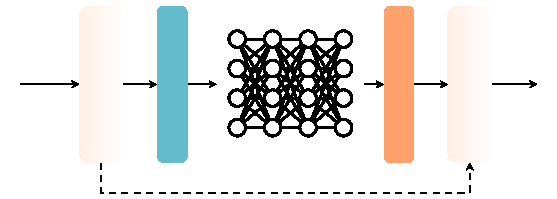
\includegraphics[width = 3cm]{figures/pictograms/basic.pdf}};

    \node[rectangle, fill = IKRBlue!20, rounded corners = 5pt, minimum width = 7cm, minimum height = 1.7cm, anchor = north west, align = left, text width = 6.2cm, visible on = <3->] (c2) at (0, -2) {novel policymix concept};

    \node[anchor = center, visible on = <3->] at (2.65,-2.85) {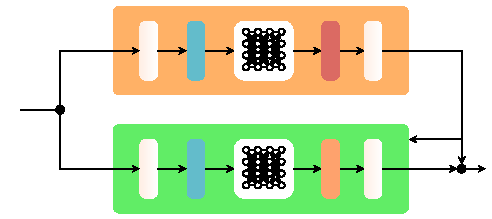
\includegraphics[width = 3cm]{figures/pictograms/policymix.pdf}};

    \node[rectangle, fill = IKRBlue!20, rounded corners = 5pt, minimum width = 7cm, minimum height = 1.7cm, anchor = north west, align = left, text width = 6.2cm, visible on = <4->] (c3) at (0, -4) {policymix concept \\ with autoencoders};

    \node[anchor = center, visible on = <4->] at (2.65,-4.85) {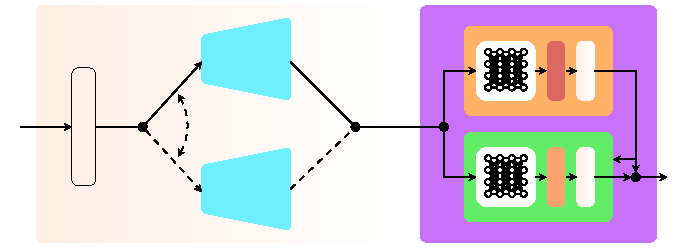
\includegraphics[width = 3cm]{figures/pictograms/aepolicy.pdf}};

    \node[rectangle, fill = greenlatte!20, rounded corners = 5pt, minimum width = 7cm, minimum height = 1.7cm, anchor = north west, align = left, text width = 6.2cm, visible on = <5->] (o1) at (4, 0) {use of other DL techniques \\ like LSTMs, Transformers, ...};

    \node[anchor = center, visible on = <5->] at (7, -0.85) {
\includegraphics[width = 1.3cm]{figures/pictograms/dlpicto.pdf}};

    \node[rectangle, fill = greenlatte!20, rounded corners = 5pt, minimum width = 7cm, minimum height = 1.7cm, anchor = north west, align = left, text width = 6.2cm, visible on = <6->] (o2) at (4, -2) {include further policies};

    \node[align = center, visible on = <6->] at (7, -2.85) {\Huge $\pi$};

    \node[rectangle, fill = greenlatte!20, rounded corners = 5pt, minimum width = 7cm, minimum height = 1.7cm, anchor = north west, align = left, text width = 6.2cm, visible on = <7->] (o3) at (4, -4) {more topologies};

    \node[anchor = center, visible on = <7->] at (7, -4.85) {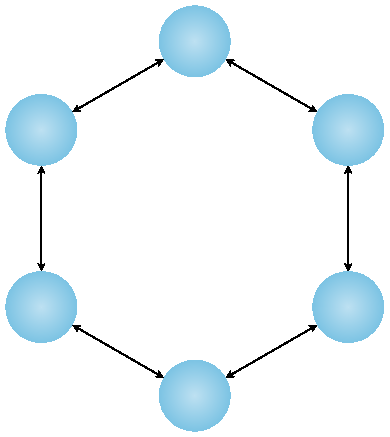
\includegraphics[width = 1.3cm]{figures/pictograms/othertopos.pdf}};

    \draw[arrowbold, shorten <= 2mm, shorten >= 2mm, visible on = <5->] (c1) -- (o1);
    \draw[arrowbold, shorten <= 2mm, shorten >= 2mm, visible on = <6->] (c2) -- (o2);
    \draw[arrowbold, shorten <= 2mm, shorten >= 2mm, visible on = <7->] (c3) -- (o3);

    %add pictograms
     
\end{tikzpicture}